\section{Модели и спецификация требований к программному средству}
\label{sec:funcreq}

\subsection{Теоритический анализ}

На основе теории рассмотренной в главе \ref{sec:domain} можно сделать выводы что задачу распознавания можно декомпозировать на следующие подзадачи применяемые последовательно:
\begin{itemize}
	\item пред-обработка;
	\item поиск номерного знака;
	\item распознание символов;
\end{itemize} 

Пре-обработка будет упоминаться в контексте остальных задач из за ее тесной связанности с ними.

\subsubsection{}
\label{seq:funcreq:analisys}
Поиск номерного знака

В разделе \ref{sub:domain:search:violajones} был рассмотрен метод Виолы - Джонса, именно его я буду использовать для нахождения номерного знака. 
\begin{figure}[ht]
\centering
  \begin{subfigure}[b]{0.48\textwidth} 
    \centering
    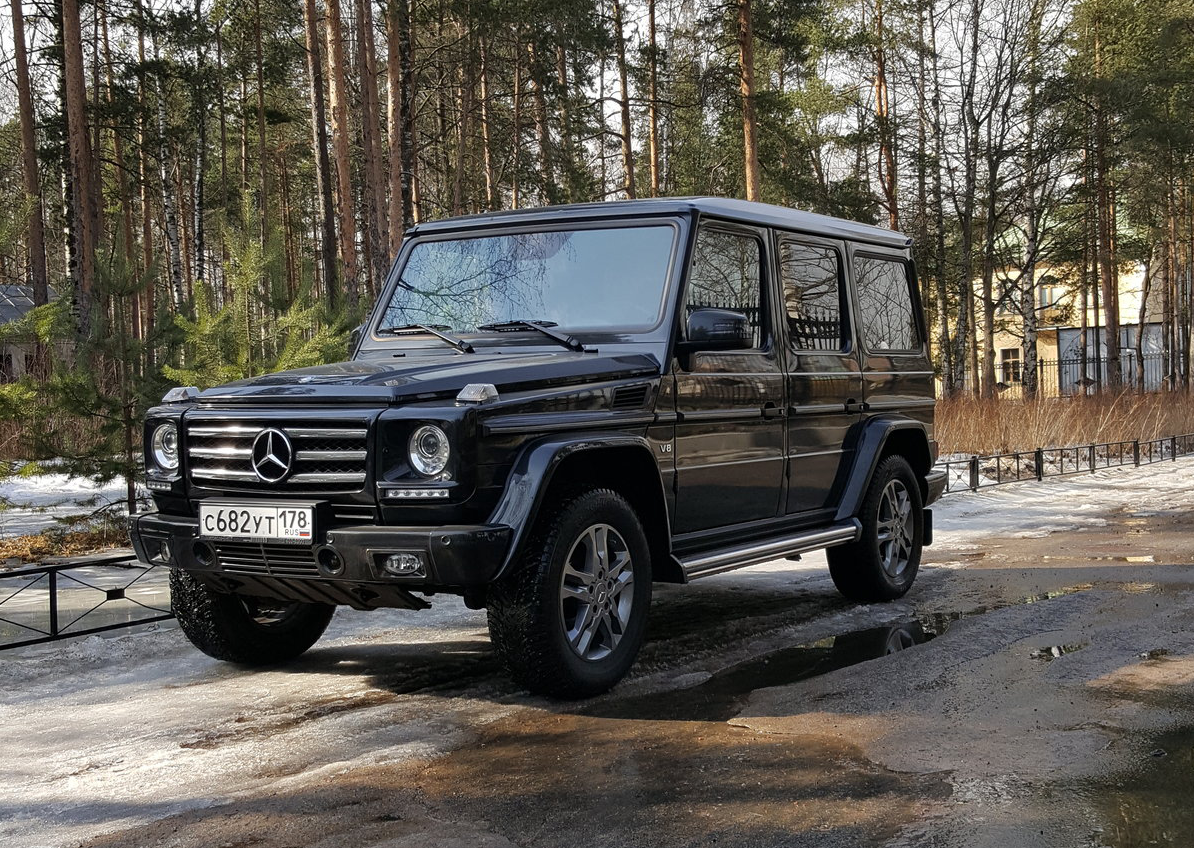
\includegraphics[width=\textwidth]{before_viola.png}  
    \caption{Исходное изображение}
  \end{subfigure}
  \begin{subfigure}[b]{0.48\textwidth} 
    \centering
    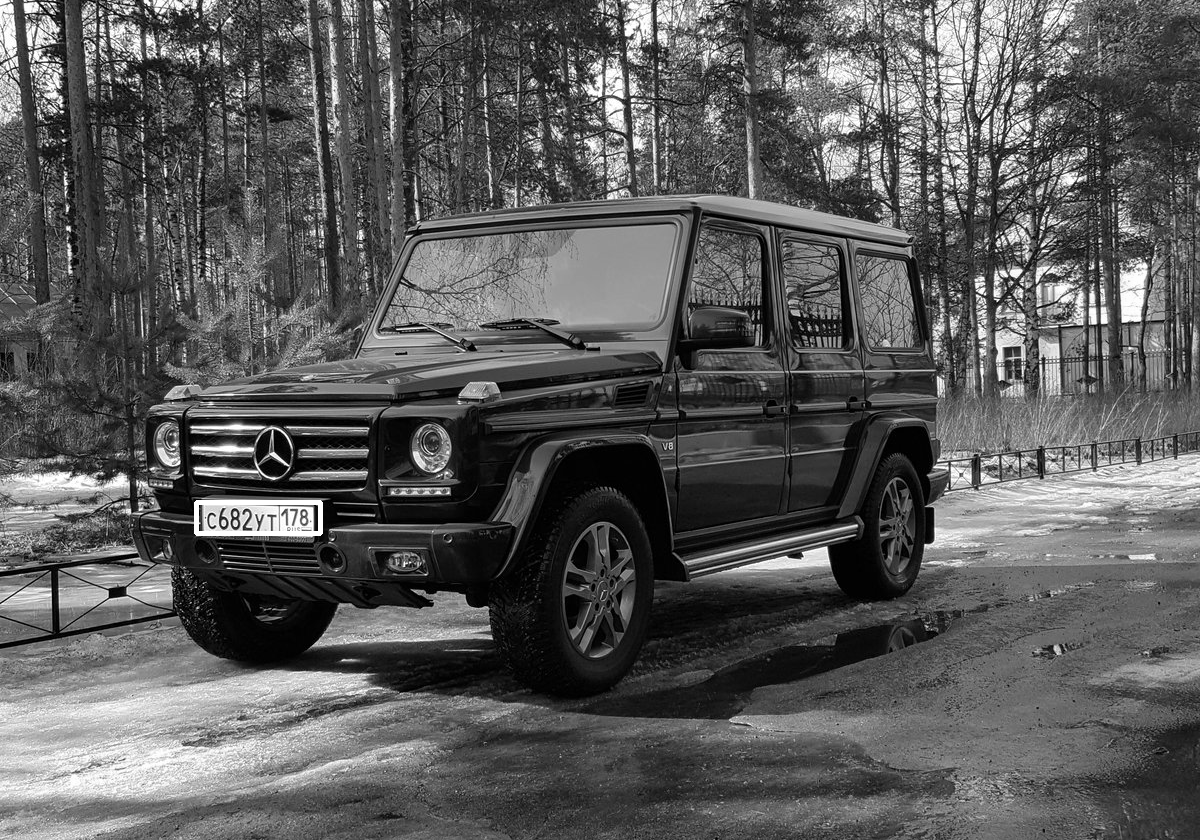
\includegraphics[width=\textwidth]{after_viola.png}  
    \caption{Обработанное изображение}
  \end{subfigure}
  \caption{Результат работы метода Виолы - Джонса}
  \label{fig:funcreq:analisys:viola}
\end{figure}
Этот алгоритм достаточно трудно реализовать, не говоря уже об эффективной реализации, поэтому целесообразно использовать его реализацию из OpenCv. Но перед его использованием его нужно научить находить номерные знаки. Для этого требуется большая база данных изображений с положительными и отрицательными примерами, а также файл-дескриптор описывающий координаты искомого объекта, по которым будет сформирован каскад Хаара, представляющий из себя xml файл c описанем примитивов Хаара и их вычисляемых значений. При разработке очень поможет тот факт что метод Виолы - Джонса распознает объекты находящиеся под углом до $30\degree$. На изображении \ref{fig:funcreq:analisys:viola} можно увидеть пример работы метода Виолы - Джонса, найденная номерная табличка была выделенна белой рамкой для наглядности. Как можно заметить хоть метод и находит изображения повернутые на угол до $30\degree$ но не определяет поворот таблички. 

\subsubsection{}
Распознавание символов

В разделе \ref{sub:domain:recognition:tesseract} был рассмотрен инструмент для распознавания текста Tesseract. Хоть он и избавляет нас от большого количества работы реализуя распознавание он не идеален, и Google дает целый список рекомендаций как повысить качество распознавания \cite{tesseract_impruvment}, не выполняя эти рекомендации процент распознанных символов крайне мал.

После работы метода Виолы - Джонса на вход модулю распознающему текст приходит вырезанная рамка автомобильного номера. И тут сталкиваемся со следующими проблемами:
\begin{itemize}
	\item текст будет под углом;
	\item неравномерные отступы;
	\item на номере присутствуют не только символы;
\end{itemize}

Прежде всего текст нужно выровнять. Эту проблему можно решать по разному. Считаю наиболее рациональным подходом найти отдельные символы затем по их координатам определить угол. На изображении \ref{fig:funcreq:analisys} изображен условный пример для поиска угла наклона. Требуется провести прямую линию параллельную символам а затем имея координаты двух любых точек по определению вычислить тангенс и найти угол $\alpha = \arctan(\frac{y_1 - y_2}{x_1 - x_2})$

\begin{figure}[ht]
\centering
    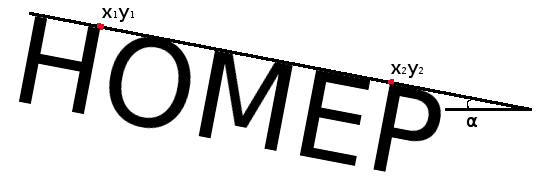
\includegraphics[scale=0.5]{find_angle.png}  
    \caption{Нахождение угла поворота таблички}
    \label{fig:funcreq:analisys}
\end{figure}

Для решения с отступами и посторонними артефактами можно попросту распознавать по одному символу, находить же символы можно по анализу контуров похожему на рассмотренный в разделе \ref{sub:domain:search:edges_analisys}. Пример работы алгоритма поиска контуров можно увидеть на изображении \ref{fig:funcreq:analisys:contour}.

\begin{figure}[ht]
\centering
  \begin{subfigure}[b]{0.48\textwidth} 
    \centering
    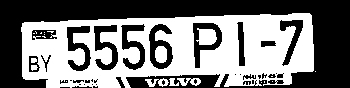
\includegraphics[width=\textwidth]{before_contour_analisys.png}  
    \caption{Исходное изображение}
  \end{subfigure}
  \begin{subfigure}[b]{0.48\textwidth} 
    \centering
    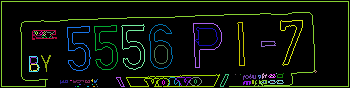
\includegraphics[width=\textwidth]{after_contour_analisys.png}  
    \caption{Обработанное изображение}
  \end{subfigure}
  \caption{Результат поиска контуров}
  \label{fig:funcreq:analisys:contour}
\end{figure}

Найти символы среди всех контуров можно проанализировав размеры каждого контура. Повернув и вырезав отдельные символы их можно передавать к Tessract. 

\subsection{Функциональная модель программного средства}
\label{sec:funcreq:funcmodel}

С оглядкой на существующие реализации рассматриваемой задачи определим варианты использования програмного средства представленных на рисунке \ref{fig:funcreq:funcmodel}.

\begin{figure}[ht]
\centering
    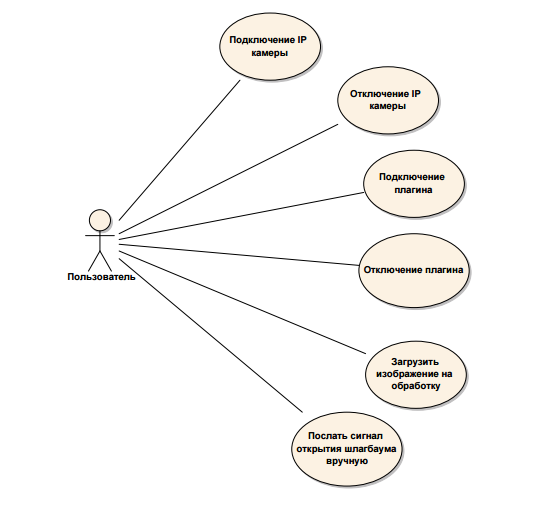
\includegraphics[scale=1]{use-case.png}  
    \caption{Диаграмма вариантов использования}
  \label{fig:funcreq:funcmodel}
\end{figure}

На основе вариантов использования для разрабатываемого программного средства формируется следующий набор функциональных требований:
\begin{itemize}
	\item Подключение и обработка видеопотока с IP камеры
	\item Отключение от IP камеры.
	\item Загрузка изображения для распознавания.
	\item Подключение плагинов обрабатывающих результаты распознавания.
	\item Отключение плагинов обрабатывающих результат распознавания.
\end{itemize}

\subsection{Спецификация требований к программному средству}
\label{sec:fucreq:specification}

\subsubsection{}
Подключение IP камер. Требования:
\begin{itemize}
	\item возможность подключится либо отключиться от камеры должна быть как с командной строки так и из пользовательского веб интерфейса;
	\item адреса добавленных IP камер должны сохранятся и при перезапуске сервера, сервер должен снова подключится к камерам;
	\item должна быть возможность добавить несколько IP камер;
	\item у каждой IP камеры кроме имени должен быть псевдоним, указываемый при подключении, который будет передаваться вместе с результатами распознавания в плагины;
\end{itemize}

\subsubsection{}
Загрузка изображений для распознавания. Требования:
\begin{itemize}
	\item Возможность загрузить изображение на сервер для распознавания
	\item Поддержка форматов PNG и JPEG
\end{itemize}


\subsubsection{}
Подключение плагинов для обработки результатов распознавания. Требования:
\begin{itemize}
	\item плагины подключаются путем копирования dll файлов в директорию plugins;
	\item для создания плагинов требуется используя библиотеку реализовать интерфейс обработчика результатов на платформе \dotnet{};
	\item плагины должны ожидать как положительный так и отрицательный результат;
\end{itemize}

\subsubsection{}
Процесс распознавания номеров. Требования:
\begin{itemize}
	\item сервер должен обрабатывать видеопоток от IP камер;
	\item при распознании номера результаты должны быть переданны подключенным плагинам;
	\item при команде открытия шлагбаума от оператора требуется передать плагинам отрицательный результат для обработки.
\end{itemize}

\subsubsection{}
Пользовательский интерфейс програмного средства.
\begin{itemize}
	\item Пользовательский интерфейс должен быть Web страницей
	\item Должны поддерживаться Google Chrome и Firefox последних версий.
	\item Должны быть возможность конфигурирования сервера через командную строку.
\end{itemize}

\subsubsection{}
Совместимость программного средства
\begin{itemize}
	\item Требуется совместимость с Windows 10
\end{itemize}